

%\documentclass{book}\begin{document}<content\end{document}
\documentclass[letter, 11pt, margins=0.25in]{texMemo}  % The texMemo package by Rob Oakes.

\usepackage{amsmath}
\usepackage[colorlinks=true, citecolor=blue]{hyperref}
\usepackage{enumitem}
\usepackage{graphicx, lipsum}

\usepackage[LGRgreek]{mathastext}

\usepackage{matlab-prettifier}

\usepackage{natbib}
\bibliographystyle{apalike}


\memodate{\today~(Submitted)}
%\memoto{Dr. Dan Russell - College of Engineering, Penn State University}
%\memofrom{Michael R. Wirtzfeld - Sound Discovery LLC\\}
\memosubject{Noise Control Applications - Module 1 Assignement\\}

%\memologo{
\includegraphics[width=1.0\textwidth]{SOUND_DISCOVERY_Business_Card.jpg}}



\begin{document}

\maketitle


\vspace{-0.25cm}
\section*{Problem 1 - Cut-on Frequencies in Ducts and Pipes}

The Matlab code for this problem is listed in Appendix~\ref{appendix:problem1}.

\vspace{-0.25cm}
\subsection*{Problem 1a}

The lowest cut-on frequency for a rectangular duct with air flow is given by equation,

\vspace{-0.25cm}
\begin{equation}
    f_{cut-on} = 0.5 \cdot \frac{c}{L}
\end{equation}

where $c$ is the speed of sound in air, 343~$\frac{m}{s}$,  and $L$ is the largest side of the rectangular cross-section.

\vspace{0.25cm}
With cross-sectional dimensions of $L_x = 12~cm$ and $L_y = 20~cm$, the lowest cut-on frequency for this rectangular duct is,

\vspace{-0.25cm}
\begin{equation*}
    f_{cut-on} = 0.5 \cdot \frac{ 343~\frac{m}{s} }{ 0.20~m } = \boldsymbol{857.5~Hz}
\end{equation*}



\vspace{-0.25cm}
\subsection*{Problem 1b}

The lowest cut-on frequency for a circular duct with air flow with the same cross-sectional area as the rectangular duct in part (a.) can be calculated using equation,

\vspace{-0.25cm}
\begin{equation}
    f_{cut-on} = 0.568 \cdot \frac{c}{d}
    \label{equation:circularDuct}
\end{equation}

where $c$ is the speed of sound in air, 343~$\frac{m}{s}$,  and $d$ is diameter of the circular duct.

\vspace{0.25cm}
The cross-sectional area of the rectangular duct is,

\vspace{-0.25cm}
\begin{equation*}
    Area_{~rectangular~duct} = 0.12~m~\cdot0.20~m =  0.024~m
\end{equation*}

\vspace{0.25cm}
The corresponding diameter for this area is,

\vspace{-0.25cm}
\begin{equation*}
    diameter = \sqrt{ \frac{0.24~m^2}{\pi} } \cdot 2 = 0.17~m
\end{equation*}

\vspace{0.25cm}
Using Eq.~\ref{equation:circularDuct}, the lowest cut-on frequency for this circular duct with air flow is,

\vspace{-0.25cm}
\begin{equation*}
    f_{cut-on} = 0.568 \cdot \frac{ 1,500~\frac{m}{s} }{ 0.17~m } = \boldsymbol{1,114.5~Hz}
\end{equation*}




\vspace{-0.25cm}
\subsection*{Problem 1c}

The lowest cut-on frequency for this circular duct with water flow can be calculated using Eq.~\ref{equation:circularDuct},

\vspace{-0.25cm}
\begin{equation*}
    f_{cut-on} = 0.568 \cdot \frac{ 1,500~\frac{m}{s} }{ 0.17~m } = \boldsymbol{4,873.9~Hz}
\end{equation*}

The lowest cut-on frequency for water is considerable larger than it is for air flow.





\newpage
\subsection*{Problem 1d}

The speed of sound in air is calculated by,

\vspace{-0.25cm}
\begin{equation}
    c = \sqrt{ \gamma \cdot R \cdot T_K }
    \label{equation:speedOfSoundInAir}
\end{equation}

where $\gamma = 1.4$ is the ratio of specific heats, $R = 287~\frac{J}{kg \cdot K}$ is the gas constant, and $T_K$ is the absolute temperature in Kelvin.

\vspace{0.25cm}
Figure~\ref{figure:cuton_frequency_versus_temperature} illustrates how the lowest cut-on frequency changes as the air heats from $0^{\circ}$ to $500^{\circ}$ Celsius.

\vspace{0.25cm}
The square-root relationship between temperature and the speed of sound in air is apparent and governs the behaviour of the cut-on frequency.




\vspace{-4.8cm}
\begin{figure}[!htb]

    \center
        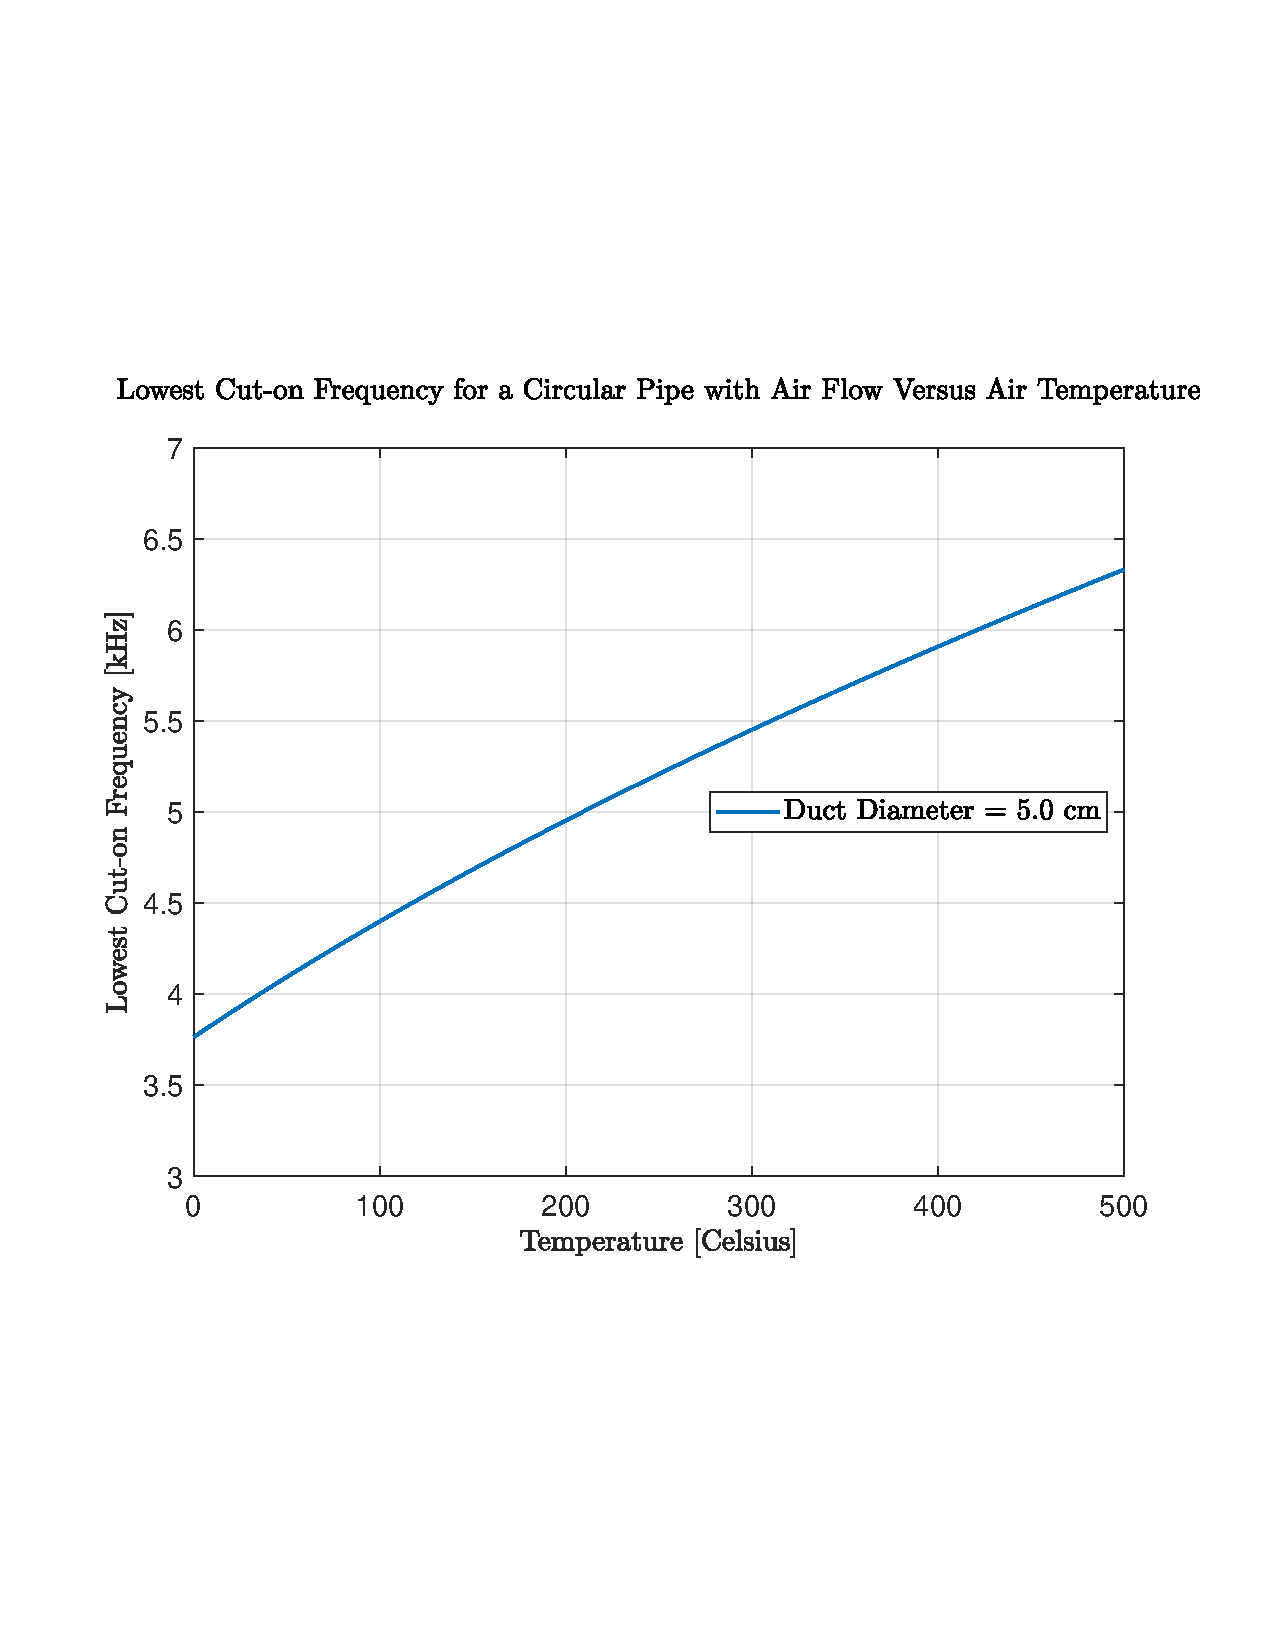
\includegraphics[ scale = 0.8, keepaspectratio ]{Cut-on Frequency Versus Temperature - Sunday, January 19, 2025.pdf}

    \vspace{-5.2cm}
    \caption{Lowest cut-on frequency for a circular 5 cm diameter duct versus air temperature.}
    \label{figure:cuton_frequency_versus_temperature}

\end{figure}





\vspace{-0.25cm}
\subsection*{Problem 1e}

 \textbf{Question:  Are cut-on frequencies higher for a circular or rectangular duct for a given cross-sectional area?}

 The lowest cut-on frequency is higher for a circular duct than for a
 rectangular duct for a given cross-sectional area.

 For the dimensions given in class, the rectangular duct is not square.
 This produces a larger dimension and thus a smaller, lowest cut-on
 frequency.  If the rectangular duct is square dimensions on the order
 of the circular duct diameter with the same cross-sectional area, the
 cut-on frequencies are approximately equal.



\vspace{0.25cm}
\textbf{Question:  What about in air versus water?}

 The lowest cut-on frequency is larger for water than for air.  The cut-on
 frequency is proportional to the speed of sound and the speed of sound in
 water is greater than the speed of sound in air.



\vspace{0.25cm}
\textbf{Question:  What about cold versus hot air?}

 The lowest cut-on frequency is higher for warm air than it is for cold air.









\newpage
\section*{Problem 2 - Muffler Design Comparison}

The Matlab code for this problem is listed in Appendix~\ref{appendix:problem2}.

For these muffler comparisons, it is assumed that there is no resistive terms and no flow.  Since transmission losses are considered, the end corrections (i.e., load impedance at outlet of the system) have no physical meaning and are not accounted for in the computations.


\vspace{-0.25cm}
\subsection*{Problems 2a, 2b, and 2c}

\vspace{-0.25cm}
Figure~\ref{figure:problem2figure1} shows the transmission loss profiles for a simple expansion chamber, a double-tuned expansion chamber, and a cascaded double-tuned expansion chamber muffler.

The peaks for the simple expansion chamber (red, dashed line) are approximately 22 dB and occur at frequencies with a wavelength that is a quarter of the length of the expansion chamber.  Minimal loss occurs at half wavelength multiples.

The addition of the extension tube inside the muffler produces a quarter wavelength resonator.  The side branch of Ji (2005;  Slide 11, Lecture 3 notes) was used to calculate $L_o$.  For the cascaded double-tuned expansion chamber, the extension tubes produce a secondary quarter wavelength resonator.

As noted in the office hours session, there is no damping which produces artificially high resonances.


\begin{figure}[!htb]

    \center
        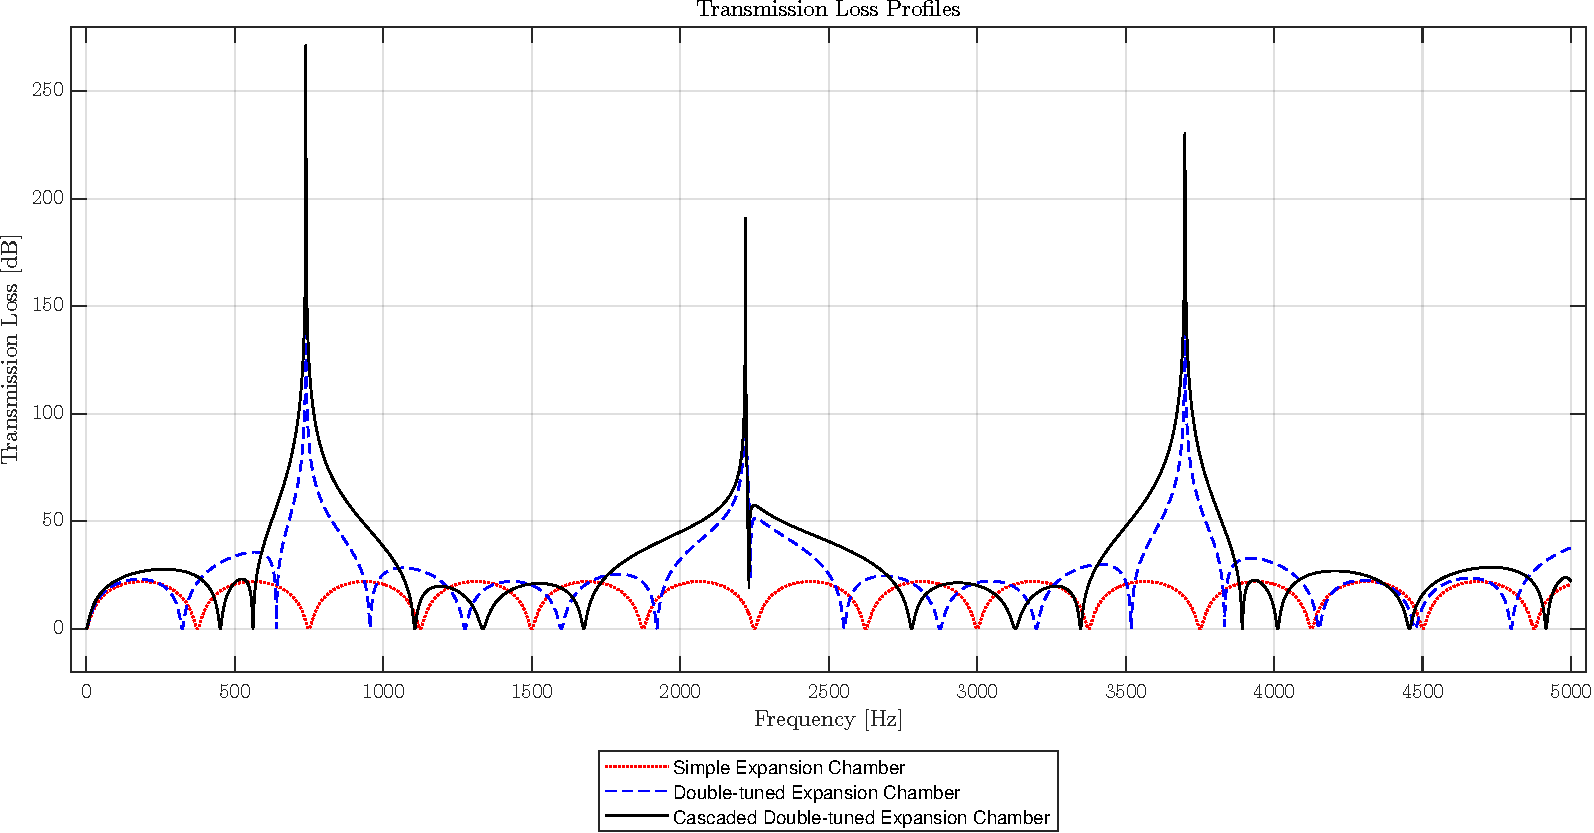
\includegraphics[ scale = 0.675, keepaspectratio ]{Assignment 1 - Question 2 Figure All TL Profiles.pdf}

    \caption{Transmission loss profiles for a simple expansion chamber, a double-tuned expansion chamber, and a cascaded double-tuned expansion chamber mufflers.}
    \label{figure:problem2figure1}

\end{figure}



\subsection*{Problem 2d}

Figure~\ref{figure:problem2figure2} shows the transmission loss profiles for a cascaded double-tuned expansion chamber, and a modified cascaded double-tuned expansion chamber muffler.

Two modifications were made to the original system:

\begin{enumerate}
  \item The left 3" extension tube in the left chamber was shortened to 2" inches, making the respective muffler section 1" longer.
  \item The left 3" extension tube in the right chamber was lengthened to 4", making the respective muffler section 1" shorter.
\end{enumerate}

\vspace{0.5cm}
\begin{figure}[!htb]

    \center
        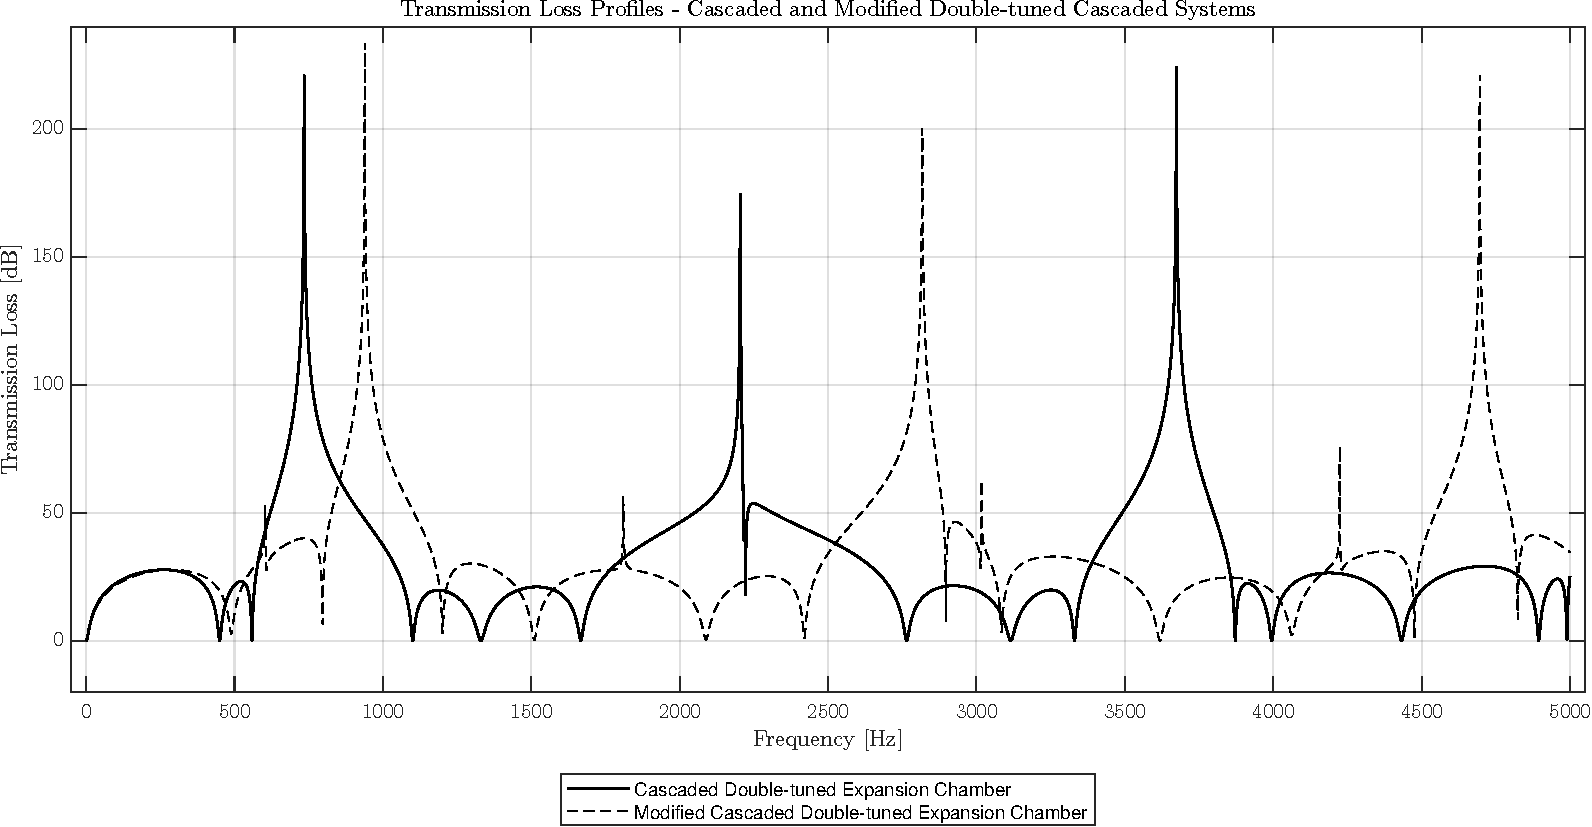
\includegraphics[ scale = 0.675, keepaspectratio ]{Assignment 1 - Question 2 Figure Comparison TL Plot For Cascaded Systems.pdf}

    \caption{Transmission loss profiles for a cascaded double-tuned expansion chamber muffler and a modified version of this muffler.}
    \label{figure:problem2figure2}

\end{figure}

\vspace{0.25cm}
These modifications change the symmetry of the cascaded system, and allow the resonate frequencies to be independently changed.












\newpage
\section*{Problem 3 - Bugle Recorder}

Diameters of holes should be smaller than a wavelength.

$R_A$ is neglected (energy loss).

\subsection*{Problem 3a}

\subsection*{Problem 3b}










\newpage
\section*{Problem 4 - Intake Duct}

\subsection*{Problem 4a}

\subsection*{Problem 4b}

\subsection*{Problem 4c}

\subsection*{Problem 4d}










\newpage
\section*{Problem 5 - Intake Duct Silencer}

\subsection*{Problem 5a}

\subsection*{Problem 5b}

\subsection*{Problem 5c}

\subsection*{Problem 5d}

\subsection*{Problem 5e}






\newpage
\section{Appendix - Matlab Code for Problem 1}
\label{appendix:problem1}

\begin{lstlisting}[style=Matlab-editor, basicstyle=\fontfamily{pcr}, numbers=none, keepspaces, mlshowsectionrules, basicstyle=\footnotesize]

%% Synopsis

% Question 1 - Cut-on Frequencies in Ducts and Pipes



%% Environment

close all; clear; clc;
% restoredefaultpath;

% addpath( genpath( '' ), '-begin' );
addpath( genpath( '../40 Assignments/00 Support' ), '-begin' );

% set( 0, 'DefaultFigurePosition', [  400  400  900  400  ] );  % [ left bottom width height ]
set( 0, 'DefaultFigurePaperPositionMode', 'manual' );
set( 0, 'DefaultFigureWindowStyle', 'normal' );
set( 0, 'DefaultLineLineWidth', 1.5 );
set( 0, 'DefaultTextInterpreter', 'Latex' );

format ShortG;

pause( 1 );

PRINT_FIGURES = 0;



%% Define Constants and Anonymous Functions

c_air = 343;  % The speed of sound in air (meters per second).
c_water = 1500;  % The speed of sound in water (meters per second).

gamma = 1.4;  % The ratio of specific heats [unitless].
R = 287;  % The gas constant [Joules per ( kilogram * Kelvin)].


h_f_cut_on_rectangular_duct = @( c, L )  0.5 .* c ./ L;
%
% c - The speed of sound.
% L - The largest cross-section dimension of the rectangular duct.


h_f_cut_on_circular_duct = @( c, d )  0.568 .* c ./ d;
%
% c - The speec of sound.
% L - The diameter of the circular duct.


h_speed_of_sound_in_air = @( gamma, R, temperature_Kelvin)  sqrt( gamma .* R .* temperature_Kelvin );



%% Problem 1a

% The cross-sectional dimensions for the rectangular duct are:  Lx = 12 cm and Ly = 20 cm.

% The largest dimension is Ly = 20 cm or 0.2 m.

% The cut-on frequency is,
h_f_cut_on_rectangular_duct( c_air, 0.2 );  % 857.5 Hz (shown in class 858 Hz)
    fprintf( 1, '\n Problem 1a:  The lowest cut-on frequency for the rectangular pipe with air is %3.1f Hz.\n', h_f_cut_on_rectangular_duct( c_air, 0.2 ) );



%% Problem 1b

% The cross-sectional dimensions for the rectangular duct are:  Lx = 12 cm and Ly = 20 cm.

% The cross-sectional area of the rectangular duct is 12 cm * 20 cm = 240 cm^2 or 0.024 m^2.
rectangular_duct_cross_sectional_area = 0.12 * 0.20;  % 0.024 m^2

% The diameter of the circulat pipe is,
circular_duct_diameter = sqrt( 0.024 / pi ) * 2;  % 0.17481 meters
%
% Check:
    % pi * ( circular_duct_diameter / 2 )^2  CHECKED


% The cut-on frequency for the circular duct is,
h_f_cut_on_circular_duct( c_air, circular_duct_diameter );  % 1,114.5 Hz
    fprintf( 1, '\n Problem 1b:  The lowest cut-on frequency for the circular pipe (of equal area) with air is %3.1f Hz.\n', h_f_cut_on_circular_duct( c_air, circular_duct_diameter ) );



%% Problem 1c

% The cut-on frequency for the circular duct with water is,
h_f_cut_on_circular_duct( c_water, circular_duct_diameter );  % 4,873.9 Hz
    fprintf( 1, '\n Problem 1c:  The lowest cut-on frequency for the circular pipe (of equal area) with water is %3.1f Hz.\n', h_f_cut_on_circular_duct( c_water, circular_duct_diameter ) );

% The cut-on frequency should be higher because it is proportional to the
% speed of sound in a given medium.



%% Problem 1d

fprintf( 1, '\n Problem 1d:  See the figure.\n' );

temperature_range_celsius = 0:0.1:500;  % Celsius
    temperature_range_kelvin = temperature_range_celsius + 273.15;  % Kelvin


FONT_SIZE = 14;

figure( ); ...
    plot( temperature_range_celsius, h_f_cut_on_circular_duct( h_speed_of_sound_in_air( gamma, R, temperature_range_kelvin ), 0.05 ) ./ 1e3 );  grid on;
        legend( 'Duct Diameter = 5.0 cm', 'Location', 'East', 'FontSize', FONT_SIZE, 'Interpreter', 'Latex' );
        set( gca, 'FontSize', FONT_SIZE );
    %
    xlabel( 'Temperature [Celsius]', 'FontSize', FONT_SIZE );
        % xl = get( gca, 'xlabel' );    pxl = get( xl, 'position' );  pxl( 2 ) = 1.1 * pxl( 2 );
        %     set( xl, 'position', pxl );
    %
    ylabel( 'Lowest Cut-on Frequency [kHz]', 'FontSize', FONT_SIZE );
        % yl = get( gca, 'ylabel' );  pyl = get( yl, 'position' );  pyl( 1 ) = 1.2 * pyl( 1 );
        %     set( yl, 'position', pyl );
    %
    caption = sprintf( 'Lowest Cut-on Frequency for a Circular Pipe with Air Flow Versus Air Temperature\n' );
        title( caption, 'FontSize', FONT_SIZE );
    %
    ylim( [ 3  7 ] );



%% Problem 1e

fprintf( 1, '\n Problem 1e:  See Section Problem 1e of the Matlab script for the answers.\n\n' );


% Question:  Are cut-on frequencies higher for a circular or rectangular duct for a given cross-sectional area?

% The lowest cut-on frequency is higher for a circular duct than for a
% rectangular duct for a given cross-sectional area.

% For the dimensions given in class, the rectangular duct is not square.
% This produces a larger dimension and thus a smaller, lowest cut-on
% frequency.

% If the rectangular duct is square dimensions on the order of the circular
% duct diameter with the same cross-sectional area, the the cut-on
% frequencies are approximately equal.


% Question:  What about in air versus water?

% The lowest cut-on frequency is larger with water than air.  This due to
% the fact that the cut-on frequency is proportional to the speed of sound
% and the speed of sound in water is greater than it is in air.


% Question:  What about cold versus hot air?

% For a circular pipe, the cut-on frequency is higher in warm air than cold
% air.



%% Clean-up

if ( ~isempty( findobj( 'Type', 'figure' ) ) )
    monitors = get( 0, 'MonitorPositions' );
        if ( size( monitors, 1 ) == 1 )
            autoArrangeFigures( 2, 2, 1 );
        elseif ( 1 < size( monitors, 1 ) )
            autoArrangeFigures( 2, 2, 1 );
        end
end


if ( PRINT_FIGURES == 1 )
    saveas( gcf, 'Cut-on Frequency Versus Temperature - Sunday, January 19, 2025.pdf' );
end


fprintf( 1, '\n\n\n*** Processing Complete ***\n\n\n' );



%% Reference(s)
\end{lstlisting}









\newpage
\section{Appendix - Matlab Code for Problem 2}
\label{appendix:problem2}

\begin{lstlisting}[style=Matlab-editor, basicstyle=\fontfamily{pcr}, numbers=none, keepspaces, mlshowsectionrules, basicstyle=\footnotesize]

%% Synopsis

% Question 2 - Muffler Design Comparison



%% Environment

close all; clear; clc;
% restoredefaultpath;

% addpath( genpath( '' ), '-begin' );
addpath( genpath( '../00 Support' ), '-begin' );

% set( 0, 'DefaultFigurePosition', [  400  400  900  400  ] );  % [ left bottom width height ]
set( 0, 'DefaultFigurePaperPositionMode', 'manual' );
set( 0, 'DefaultFigureWindowStyle', 'normal' );
set( 0, 'DefaultLineLineWidth', 1.5 );
set( 0, 'DefaultTextInterpreter', 'Latex' );

format ShortG;

pause( 1 );

PRINT_FIGURES = 0;



%% Constants

rho0 = 1.21;  % Ratio of specific heats (unitless).
c = 343;  % Speed of sound in air (meters per second).

frequency_set = 0:1:5e3;  % Hertz



%% Dimensions

convert.inches_to_meters = 0.0254;
convert.foot_to_meters = 0.3048;

dimensions.inlet_diameter_meters = 2 * convert.inches_to_meters;  % 0.0508 meters
dimensions.inlet_length_meters = 6 * convert.foot_to_meters;  % 1.82 meters

dimensions.muffler_diameter_meters = 10 * convert.inches_to_meters;  % 0.254 meters
dimensions.muffler_length_meters = 18 * convert.inches_to_meters;  % 0.4572 meters

dimensions.outlet_diameter_meters = 2 * convert.inches_to_meters;  % 0.0508 meters
dimensions.outlet_length_meters = 1 * convert.foot_to_meters;  % 0.3048 meters

outlet_flanged = false;

dimensions.overhang = 3 *convert.inches_to_meters;  % 0.0762 meters

segment_diameters = [ ...
    dimensions.outlet_diameter_meters, ...
    dimensions.muffler_diameter_meters, ...
    dimensions.inlet_diameter_meters, ...
    ].';
%
h_area_from_diameter = @( d )  pi .* d.^2 ./ 4;
%
segment_areas = h_area_from_diameter( segment_diameters );

segment_lengths = [ ...
    dimensions.outlet_length_meters, ...
    dimensions.muffler_length_meters, ...
    dimensions.inlet_length_meters, ...
    dimensions.overhang, ...
    ].';



%% Part a - Simple Expansion Chamber

nFreq = length( frequency_set );
    TL = zeros( nFreq, 1 );

for frequency_index = 1:1:nFreq

    f = frequency_set( frequency_index );

    T_total = [ 1 0; 0 1 ];

    T_outlet = duct_segment_transfer_matrix( f, rho0, c, segment_lengths( 1 ), segment_areas ( 1 ) );
    T_muffler = duct_segment_transfer_matrix( f, rho0, c, segment_lengths( 2 ), segment_areas( 2 ) );
    T_inlet = duct_segment_transfer_matrix( f, rho0, c, segment_lengths( 3 ), segment_areas( 3 ) );

    T_net = T_inlet * T_muffler * T_outlet * T_total;

    T11 = T_net(1, 1);  T12 = T_net(1, 2);  T21 = T_net(2, 1);  T22 = T_net(2, 2);

    % Z = open_end_impedance( f, rho0, c, segment_lengths( 1 ), segment_areas( 1 ), outlet_flanged );
        TL( frequency_index ) = 10 * log10( abs( ( T11  +  segment_areas(3)*T12/(rho0*c)  +  (rho0*c)*T21/segment_areas(1)  +  T22 ) / 2 )^2 );

end

TL_parta = TL;



%% Part b - Double-tuned Expansion Chamber

annulus_area_squared_meters = pi/4 * ( segment_diameters(2)^2 - segment_diameters(1)^2 );
    branch_diameter = sqrt( 4 * annulus_area_squared_meters / pi );
        a = branch_diameter / 2;

epsilon = branch_diameter / segment_diameters(2);  % 0.9787
    L_o = a * ( 0.9326 - 0.6196*epsilon );  % Using Ji (2005) - Slide 11, Lecture 3 notes.


nFreq = length( frequency_set );
    TL = zeros( nFreq, 1 );

for frequency_index = 1:1:nFreq

    f = frequency_set( frequency_index );

    T_total = [ 1 0; 0 1 ];

    T_outlet = duct_segment_transfer_matrix( f, rho0, c, segment_lengths( 1 ), segment_areas ( 1 ) );
    T_muffler = duct_segment_transfer_matrix( f, rho0, c, segment_lengths(2) - 2*segment_lengths(4), segment_areas( 2 ) );
    T_inlet = duct_segment_transfer_matrix( f, rho0, c, segment_lengths( 3 ), segment_areas( 3 ) );

    k = 2*pi*f/c;
        Z_A = -1j*rho0*c/annulus_area_squared_meters*cot(k * ( dimensions.overhang + L_o ) );
            T_branch_1 = [ 1  0;  1/Z_A  1 ];
            T_branch_2 = [ 1  0;  1/Z_A  1 ];

    T_net = T_inlet * T_branch_2 * T_muffler * T_branch_1 * T_outlet * T_total;
        T11 = T_net(1, 1);  T12 = T_net(1, 2);  T21 = T_net(2, 1);  T22 = T_net(2, 2);

    % Z = open_end_impedance( f, rho0, c, segment_lengths( 1 ), segment_areas( 1 ), outlet_flanged );
        TL( frequency_index ) = 10 * log10( abs( ( T11  +  segment_areas(3)*T12/(rho0*c)  +  (rho0*c)*T21/segment_areas(1)  +  T22 ) / 2 )^2 );

end

TL_partb = TL;



%% Part c - Cascaded, Double-tuned Expansion Chamber

nFreq = length( frequency_set );
    TL = zeros( nFreq, 1 );

for frequency_index = 1:1:nFreq

    f = frequency_set( frequency_index );

    T_total = [ 1 0; 0 1 ];

    T_outlet = duct_segment_transfer_matrix( f, rho0, c, segment_lengths( 1 ), segment_areas ( 1 ) );
    T_muffler_1 = duct_segment_transfer_matrix( f, rho0, c, ( segment_lengths(2) - 4*segment_lengths(4) )/2, segment_areas( 2 ) );

    T_muffler_2 = duct_segment_transfer_matrix( f, rho0, c, ( segment_lengths(2) - 4*segment_lengths(4) )/2, segment_areas( 2 ) );
    T_inlet = duct_segment_transfer_matrix( f, rho0, c, segment_lengths( 3 ), segment_areas( 3 ) );

    k = 2*pi*f/c;
        Z_A = -1j*rho0*c/annulus_area_squared_meters*cot(k * ( dimensions.overhang + L_o ) );
            T_branch_1 = [ 1  0;  1/Z_A  1 ];
            T_branch_2 = [ 1  0;  1/Z_A  1 ];
            T_branch_3 = [ 1  0;  1/Z_A  1 ];
            T_branch_4 = [ 1  0;  1/Z_A  1 ];

    T_net = T_inlet * T_branch_4 * T_muffler_2 * T_branch_3 * T_branch_2 * T_muffler_1 * T_branch_1 * T_outlet * T_total;
        T11 = T_net(1, 1);  T12 = T_net(1, 2);  T21 = T_net(2, 1);  T22 = T_net(2, 2);

    % Z = open_end_impedance( f, rho0, c, segment_lengths( 1 ), segment_areas( 1 ), outlet_flanged );
        TL( frequency_index ) = 10 * log10( abs( ( T11  +  segment_areas(3)*T12/(rho0*c)  +  (rho0*c)*T21/segment_areas(1)  +  T22 ) / 2 )^2 );

end

TL_partc = TL;



%% Part d - Cascaded, Double-tuned Expansion Chamber

nFreq = length( frequency_set );
    TL = zeros( nFreq, 1 );

for frequency_index = 1:1:nFreq

    f = frequency_set( frequency_index );

    T_total = [ 1 0; 0 1 ];

    T_outlet = duct_segment_transfer_matrix( f, rho0, c, segment_lengths( 1 ), segment_areas ( 1 ) );
    T_muffler_1 = duct_segment_transfer_matrix( f, rho0, c, 0.1016, segment_areas( 2 ) );  % Changed to 4 inches.
    T_muffler_2 = duct_segment_transfer_matrix( f, rho0, c, 0.0508, segment_areas( 2 ) );  % Changed to 2 inches.
    T_inlet = duct_segment_transfer_matrix( f, rho0, c, segment_lengths( 3 ), segment_areas( 3 ) );

    k = 2*pi*f/c;
        Z_A = -1j*rho0*c/annulus_area_squared_meters*cot(k * ( 0.0508 + L_o ) );  % Changed to 2 inches.
            T_branch_1 = [ 1  0;  1/Z_A  1 ];
            T_branch_2 = [ 1  0;  1/Z_A  1 ];
            T_branch_4 = [ 1  0;  1/Z_A  1 ];
        %
        Z3 = -1j*rho0*c/annulus_area_squared_meters*cot(k * ( 0.1016 + L_o ) );  % Changed to 4 inches.
            T_branch_3 = [ 1  0;  1/Z3  1 ];

    T_net = T_inlet * T_branch_4 * T_muffler_2 * T_branch_3 * T_branch_2 * T_muffler_1 * T_branch_1 * T_outlet * T_total;
        T11 = T_net(1, 1);  T12 = T_net(1, 2);  T21 = T_net(2, 1);  T22 = T_net(2, 2);

    % Z = open_end_impedance( f, rho0, c, segment_lengths( 1 ), segment_areas( 1 ), outlet_flanged );
        TL( frequency_index ) = 10 * log10( abs( ( T11  +  segment_areas(3)*T12/(rho0*c)  +  (rho0*c)*T21/segment_areas(1)  +  T22 ) / 2 )^2 );

end

TL_partd = TL;



%% Plot Transmission Loss Profiles

Y_LIMITS = [ -20  240 ];

h_figure_1 = figure( ); ...
    plot( frequency_set, TL_parta, 'LineWidth', 1.0, 'LineStyle', ':', 'Color', 'r' );  hold on;
    plot( frequency_set, TL_partb, 'LineWidth', 0.9, 'LineStyle', '--', 'Color', 'b' );
    plot( frequency_set, TL_partc, 'LineWidth', 0.9, 'LineStyle', '-', 'Color', 'k' );  grid on;
        legend( ...
            'Simple Expansion Chamber', ...
            'Double-tuned Expansion Chamber', ...
            'Cascaded Double-tuned Expansion Chamber', ...
            'Location', 'SouthOutside' );
    xlabel( 'Frequency [Hz]' );  ylabel( 'Transmission Loss [dB]' );
    title( 'Transmission Loss Profiles' );
    %
    Ax = gca;
        Ax.XAxis.TickLabelInterpreter = 'latex';
        Ax.YAxis.TickLabelInterpreter = 'latex';
    %
    axis( [ -50  5e3+50  Y_LIMITS ] );


Y_LIMITS = [ -20  240 ];

h_figure_2 = figure( ); ...
    plot( frequency_set, TL_partc, 'LineWidth', 1.0, 'LineStyle', '-', 'Color', 'k' );  hold on;
    plot( frequency_set, TL_partd, 'LineWidth', 0.6, 'LineStyle', '--', 'Color', 'k' );  grid on;
        legend( ...
            'Cascaded Double-tuned Expansion Chamber', ...
            'Modified Cascaded Double-tuned Expansion Chamber', ...
            'Location', 'SouthOutside' );
    xlabel( 'Frequency [Hz]' );  ylabel( 'Transmission Loss [dB]' );
    title( 'Transmission Loss Profiles - Cascaded and Modified Double-tuned Cascaded Systems' );
    %
    Ax = gca;
        Ax.XAxis.TickLabelInterpreter = 'latex';
        Ax.YAxis.TickLabelInterpreter = 'latex';
    %
    axis( [ -50  5e3+50  Y_LIMITS ] );



%% Clean-up

if ( ~isempty( findobj( 'Type', 'figure' ) ) )
    monitors = get( 0, 'MonitorPositions' );
        if ( size( monitors, 1 ) == 1 )
            autoArrangeFigures( 2, 2, 1 );
        elseif ( 1 < size( monitors, 1 ) )
            autoArrangeFigures( 2, 2, 1 );
        end
end


if ( PRINT_FIGURES == 1 )
        exportgraphics( h_figure_1, 'Assignment 1 - Question 2 Figure All TL Profiles.pdf', 'Append', true );
        exportgraphics( h_figure_2, 'Assignment 1 - Question 2 Figure Comparison TL Plot For Cascaded Systems.pdf', 'Append', true );
end


fprintf( 1, '\n\n\n*** Processing Complete ***\n\n\n' );



%% Reference(s)
\end{lstlisting}








\end{document}






% Reference(s):

% https://tex.stackexchange.com/questions/180222/how-to-change-font-size-for-specific-lstlisting


































